\chapter{Appendix}
\section{Source alignment}\label{sec:source-alignment}
\begin{figure}
	\centering
		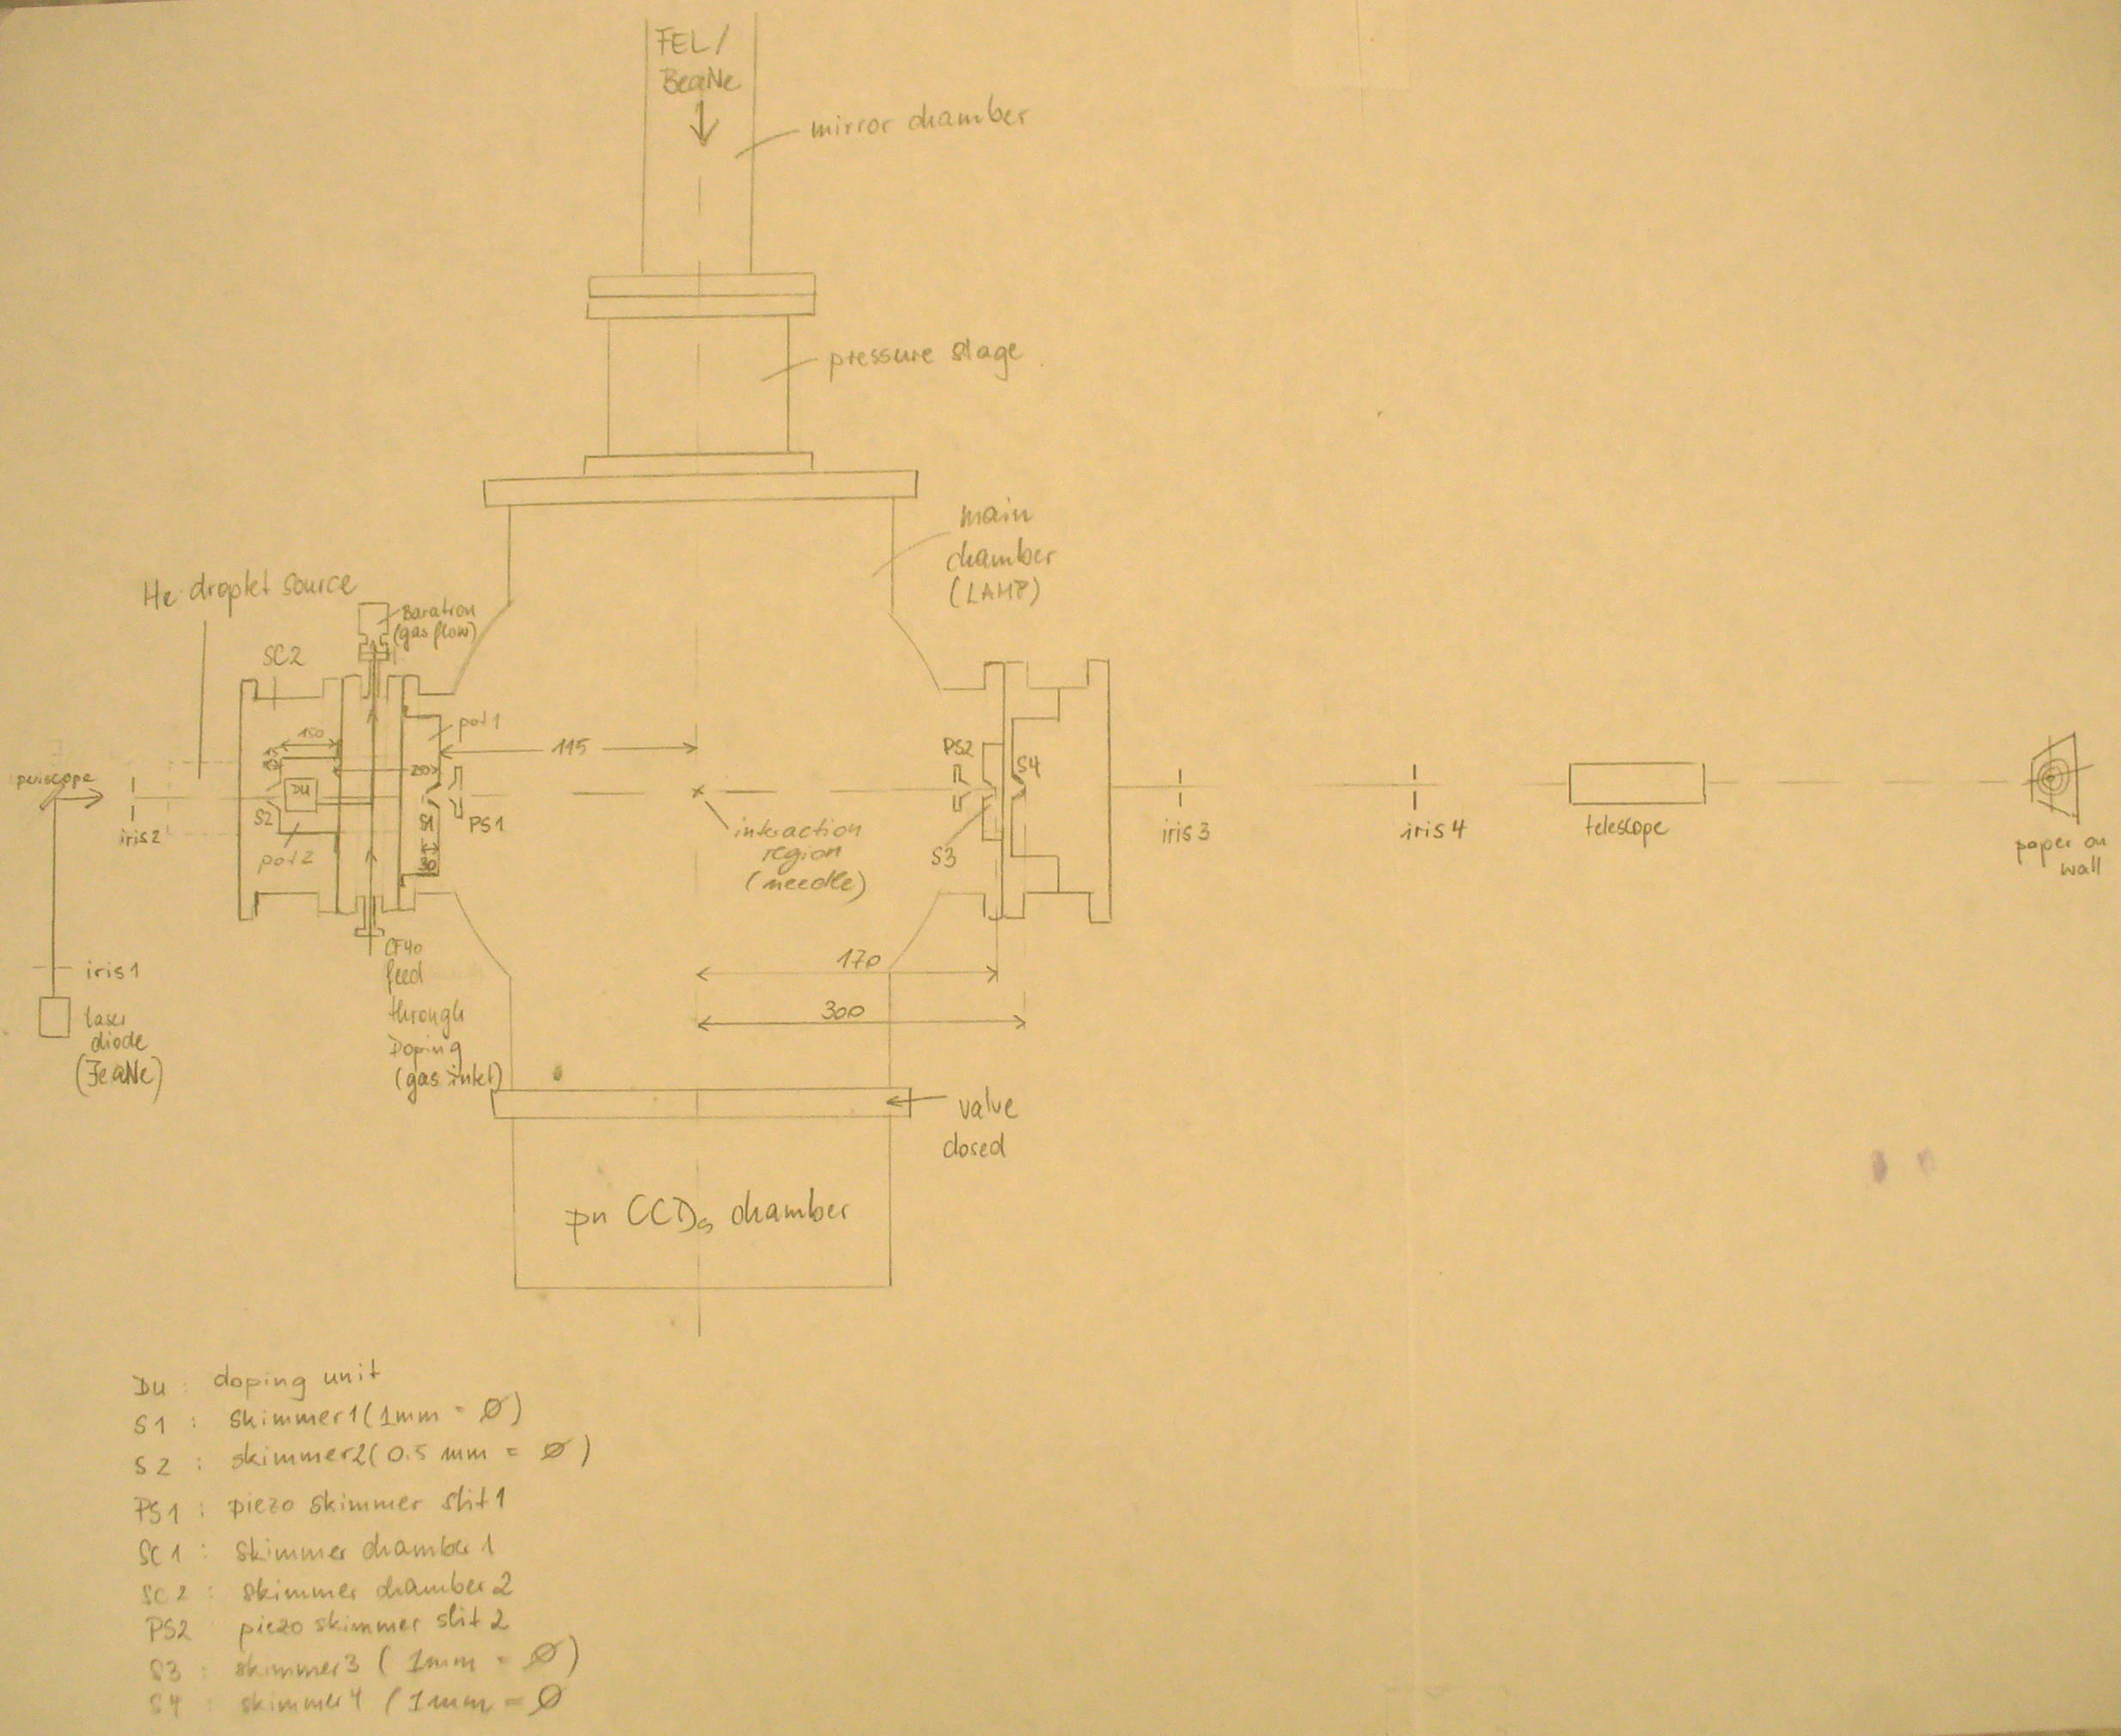
\includegraphics[width=1.00\textwidth]{images/Overview_Setup_Jetalignment.jpg}
	\caption{caption}
	\label{fig:Overview_Setup_Jetalignment}
\end{figure}
%
%
%
\section{Python code psana example}\label{sec:python-example}
Per popular request, a small analysis example is discussed\footnote{Programming languages change their syntax often, it is therefore useful to visit the web-page\\ \url{https://confluence.slac.stanford.edu/display/PSDM/LCLS+Data+Analysis}}. To begin, you should verify that you have a SLAC unix account and a SSH terminal with -Y flag capabilities\footnote{If you have problems with graphics visualization, try the following link\\ \url{https://confluence.slac.stanford.edu/display/PCDS/Remote+Visualization}}. To access the psana computer cluster, see the following commands
\begin{lstlisting}[language=csh,basicstyle=\footnotesize]
	$ ssh -Y USERNAME@pslogin.slac.stanford.edu
	$ ssh -Y psana
	$ source /reg/g/psdm/etc/ana_env.csh
\end{lstlisting}
This logs you into the SLAC psana server and loads the psana framework. Once logged in, make yourself familiar with the following python code ‘psmonLocal.py’. ‘psmonLocal.py’ has been created by Chris O'Grady for demonstration purposes and more information can be found under\\
\url{https://confluence.slac.stanford.edu/display/PSDM/Visualization+Tools}
\lstinputlisting[language=Python,frame=single,basicstyle=\footnotesize]{manuals/psmonLocal.py}
This script demonstrates a pixel detector image (CSpad) and an XY-Plot. Finally, run the script like any python script with
\begin{lstlisting}[language=csh]
	$ python /reg/g/psdm/tutorials/examplePython/psmonLocal.py
\end{lstlisting}
An interesting aspect to the python interaction is the 'TAB' method, where one can code without reading the documentation. Here a user should be on the psana servers and start ipython as follows
\begin{lstlisting}[language=csh,basicstyle=\footnotesize]
	$ ipython
\end{lstlisting}
\begin{lstlisting}[language=Python,basicstyle=\footnotesize]
	$ from psana import *
	$ ds = DataSource('exp=amotut13:run=206')
	$ det = Detector('AmoETOF.0:Acqiris.0')
	$ det.   (NOTE: user hits <TAB> after typing the "." to get list of available methods)
	$ evt = ds.events().next()    (NOTE: getting an event, since the above "Definition" line requires it)
	$ print det.waveform(evt)     (NOTE: calling the "waveform" method as required by the above "Definition" line)
\end{lstlisting}
TBD
%
%
%
\section{Matlab code on spherical integrations}\label{sec:spherical-integration}
Excerpt of the Matlab code that has been used to reduce 2D diffraction images to 1D arrays with the intensity as a function of the scattering vector $\vec{Q}$.
\begin{lstlisting}[language=matlab,frame=single,basicstyle=\footnotesize]
%%% CENTER OF HIT
x_center=xLen/2; % Actually Y-center
y_center=yLen/2; % Actually X-center
for r=(1:1500)
    %looping over points
    for y=(1:yLen)
     for x=(1:xLen)
        %check if in circle
         if (x - x_center)^2 + (y - y_center)^2 < r^2
             %norm
             rnorm(r)=rnorm(r)+1;
             % testing for noise/photons
             if rearpnccd(x,y)>0
              circleSum(r)=circleSum(r)+rearpnccd(x,y);
             end
         elseif (x - x_center)^2 + (y - y_center)^2 == r^2
             %norm
             rnorm(r)=rnorm(r)+(1/2);
             % testing for noise/photons
             if rearpnccd(x,y)>0
               circleSum(r)=circleSum(r)+(rearpnccd(x,y)/2);
             end
         end
     end
    end
    if rnorm(r)==0
        rnorm(r)=1;
    end
    if r==1
        plotSum(r)=circleSum(r)/rnorm(r);
    elseif rnorm(r)-rnorm(r-1)>0
        plotSum(r)=(circleSum(r)-circleSum(r-1))/(rnorm(r)-rnorm(r-1));
    else
        plotSum(r)=0;
    end
end
\end{lstlisting}
%
%
%
\section{Python code on 1D phase-retrieval}\label{sec:1d-phase-retrieval-code}
An excerpt of the python code that has been used to iteratively retrieve the complex fields of the diffraction pattern.
\begin{lstlisting}[language=Python,frame=single,basicstyle=\footnotesize]
# fft
for i in range(1,160):
	print i
	# Fourier Transform to Fourier Space
	fourierSpace = np.fft.fft(realSpaceAdjusted)
	# Get Phase in Fourier Space
	phase = np.exp(np.angle(fourierSpace)*I)
	# Take abslute measurement and multiply with phase
	##fourierSpaceAdjusted = abs(target)*phase
	fourierSpaceAdjusted = abs(np.concatenate((target[0:len(phasedAmplitudes)],fourierSpace[len(phasedAmplitudes):len(phasedAmplitudes)*3],target[len(phasedAmplitudes)*3:len(target)]),axis=0))*phase
	#fourierSpaceAdjusted[fourierSpaceAdjusted[len(phasedAmplitudes):len(phasedAmplitudes)*3] > phasedAmplitudes[len(phasedAmplitudes)-1]] = phasedAmplitudes[len(phasedAmplitudes)-1]
	#print len(fourierSpace)==len(fourierSpaceAdjusted)==len(phase)
	# Calculate Error in Fourier Space
	errorDiffraction = np.append(errorDiffraction,np.std(abs(fourierSpace[0:len(phasedAmplitudes)]) - abs(target[0:len(phasedAmplitudes)])))
	###
	# Fourier Transform to Real Space
	realSpace = np.fft.ifft(fourierSpaceAdjusted)
	realSpaceAdjusted = realSpace.real
	#print len(realSpace)==len(realSpaceAdjusted)
	# Set values to zero where object not expected
	#realSpaceAdjusted[30:len(realSpaceAdjusted)-30] = np.zeros(len(realSpaceAdjusted)-60)
	realSpaceAdjusted[realSpaceAdjusted < 0] = 0
	# Claculate error of Support
	errorSupport = np.append(errorSupport,np.sum(abs(np.fft.ifftshift(realSpace)[0:len(realSpace)/2 - 30])))
	#print errorSupport
\end{lstlisting}
%
%
%
\section{Python code on combining detectors}
Python code that has been used to combine pnCCD detectors.
\begin{lstlisting}[language=Python,frame=single,basicstyle=\footnotesize]
# -*- coding: utf-8 -*-
import numpy as np
import h5py
import matplotlib.pyplot as plt
from matplotlib.colors import LogNorm
from scipy import interpolate
from random import random
from scipy import ndimage

import argparse
parser = argparse.ArgumentParser()
parser.add_argument("hit", help="number of hit", type=int)
args = parser.parse_args()


############# Things to adjust per shot
### Path to data
dirPath ='/Users/Max/ownCloud/Doktor/amoa1214/combined-diffraction-patterns/r0108'+'/'             # NO "/"" at the end
hitList =np.loadtxt(dirPath+'datalist.txt', dtype="string")
pathToHDF5 = dirPath+hitList[args.hit] #there is a name bug in a previous piece of code.

### Gaps between front top pnCCD and front bottom pnCCD to the middle of the rear pnCCD.
gapTop =228
gapBot =210

### Center of the rear pnCCD (for simulation)                           
xCenter =-4                                    # offset meshgrid.
yCenter =-4

### offset between rear and front pnCCDs 
xShift =2

### Data about the cluster
clusterSize =3.04*10**-8                        # must be float
clusterInt = 0.1#390239.0*10**43                     # must be float

overlapCheck=0
############# 

############## Things to adjust per run/experiment
pixelSizePnccd =75*10**-6 					# Size of a pixel in meter.

distanceOfRearPnccd =0.74					# Distance from IR to front pnCCD in meter.
distanceOfFrontPnccd =0.36			

gainRearPnccd =1./64.						# Detector muiltiplier for gain calibration.
gainFrontPnccd =1.

scatteredWaveLength =1.5*10**-9			# Wavelength of the scattered photons in meter.

############# Program specific things
### Variables
I = 1j

### Functions
# q vector function
def qVector(pixel, pixelSize, distanceToDetector, waveLength):
	return 4.*np.pi*np.sin(np.arctan(pixel*pixelSize/distanceToDetector)/2.)/waveLength

# downsampling image
def blockMean(ar, fact):
    assert isinstance(fact, int), type(fact)
    sx, sy = ar.shape
    X, Y = np.ogrid[0:sx, 0:sy]
    regions = sy/fact * (X/fact) + Y/fact
    res = ndimage.mean(ar, labels=regions, index=np.arange(regions.max() + 1))
    res.shape = (sx/fact, sy/fact)
    return res

# Gunier's Eqn (intensity of diffraction from a sphere)
def gunEqn(qQ, A, rR):
    return A*(4*np.pi/3)**2 *rR**6 *(3*(np.sin(rR*qQ) - rR*qQ*np.cos(rR*qQ))/(rR*qQ)**3)**2

# Gunier's Eqn (amplitude of diffraction from a sphere)
def gunEqnAmpl(qQ, A, rR):
    return np.sqrt(A)*(4*np.pi/3) *rR**3 *(3*(np.sin(rR*qQ) - rR*qQ*np.cos(rR*qQ))/(rR*qQ)**3)


### Reading detectors
dataFrontTopPnccd =np.array(h5py.File(pathToHDF5,'r')['/data/FrontPnCCDLab'])[0:512,0:1023]
dataRearPnccd =np.array(h5py.File(pathToHDF5,'r')['/data/RearPnCCDLab'])
dataFrontBottomPnccd =np.array(h5py.File(pathToHDF5,'r')['/data/FrontPnCCDLab'])[531:1043,0:1023]

intRear =dataRearPnccd
intFrontTop =dataFrontTopPnccd
intFrontBottom =dataFrontBottomPnccd

# qYFrontTop, qXFrontTop =qVector(np.array(np.mgrid[(512+gap):gap:-1,-(len(dataFrontTopPnccd[0]))/2:(len(dataFrontTopPnccd[0]))/2]),pixelSize=pixelSizePnccd, distanceToDetector=distanceOfFrontPnccd, waveLength=scatteredWaveLength)
# qYFrontBottom, qXFrontBottom =qVector(np.array(np.mgrid[-gap:(-512-gap):-1,-(len(dataFrontBottomPnccd[0]))/2:(len(dataFrontBottomPnccd[0]))/2]),pixelSize=pixelSizePnccd, distanceToDetector=distanceOfFrontPnccd, waveLength=scatteredWaveLength)

### Converting Pixels to scattering vector for rear detector
qYRear, qXRear =qVector(np.array(np.mgrid[-(len(dataRearPnccd)-yCenter)/2:(len(dataRearPnccd)+yCenter)/2,
    -(len(dataRearPnccd[0]-xCenter))/2:(len(dataRearPnccd[0]+xCenter))/2]),pixelSize=pixelSizePnccd, distanceToDetector=distanceOfRearPnccd, waveLength=scatteredWaveLength)


### Creating gap mask for rear pnCCD
invertMaskRear = np.array(intRear==0, dtype='float32')


### Intensity normalization
intRear =intRear*(1/gainRearPnccd)*(distanceOfRearPnccd**2)*(1/distanceOfFrontPnccd**2)
intRear[intRear<15*(1/gainRearPnccd)*(distanceOfRearPnccd**2)*(1/distanceOfFrontPnccd**2)] =0.0          # Offset

intFrontTop[intFrontTop<350] =0.0                   # Offset

intFrontBottom[intFrontBottom<350] =0.0             # Offset

### Interpolating 'pnCCD-gap' data back detector
intRear +=gunEqn((np.sqrt(qYRear**2+qXRear**2))+0.01, clusterInt, clusterSize)*invertMaskRear

### Combining front detector
ztop =np.concatenate((intFrontTop,np.zeros((gapTop+gapBot,1023)),intFrontBottom))


### Creating downsampled array
intRearDownSmpld = blockMean(intRear, 2)
invertMaskRearDownSmpld = blockMean(invertMaskRear, 2)

y_top, x_top = intFrontTop.shape
y_bottom, x_bottom = intFrontTop.shape
y_rear, x_rear = intRearDownSmpld.shape
zy_top, zx_top =ztop.shape

intRearDownSmpldReshp = np.concatenate((np.zeros((y_top-((y_rear/2)-gapTop),x_top)),
    np.concatenate((np.zeros((y_rear,(x_rear/2)+xShift)),intRearDownSmpld,np.zeros((y_rear,(x_rear/2)-xShift-1))), axis=1),
    np.zeros((y_bottom-((y_rear/2)-gapBot),x_bottom))))

### Creating combined mask to reflect artifical pixel
invertMaskCombined =np.concatenate((np.zeros((y_top-((y_rear/2)-gapTop),x_top)),
    np.concatenate((np.ones((y_rear,x_rear/2)),invertMaskRearDownSmpld,np.ones((y_rear,x_rear/2 -1))), axis=1),
    np.zeros((y_bottom-((y_rear/2)-gapBot),x_bottom))))

### Converting Pixels to scattering vector for combined array
qYComb, qXComb =qVector(np.array(np.mgrid[-(len(invertMaskCombined)-yCenter)/2:(len(invertMaskCombined)+yCenter)/2,
    -(len(invertMaskCombined[0]-xCenter))/2:(len(invertMaskCombined[0]+xCenter))/2]),pixelSize=pixelSizePnccd, distanceToDetector=distanceOfFrontPnccd, waveLength=scatteredWaveLength)

### Creating model and phase space
#int
ampSimulatedCombinedArray =gunEqnAmpl((np.sqrt(qYComb**2+qXComb**2))+0.01, clusterInt, clusterSize)

#phase
phaseSimulatedCombinedArray =np.exp(np.angle(ampSimulatedCombinedArray)*I)


### Plotting
z_min, z_max = 0.1, intRear.max()

#plt.subplot(2,1,1)
#plt.pcolormesh(qXRear, qYRear, intRear, norm=LogNorm(vmin=z_min, vmax=z_max), cmap='plasma')
#plt.pcolormesh(qXFrontTop, qYFrontTop, intFrontTop, norm=LogNorm(vmin=z_min, vmax=z_max), cmap='plasma')
#plt.pcolormesh(qXFrontBottom, qYFrontBottom, intFrontBottom, norm=LogNorm(vmin=z_min, vmax=z_max), cmap='plasma')
#plt.colorbar()

#plt.imshow(znew, norm=LogNorm(vmin=z_min, vmax=z_max), cmap='plasma')
#plt.colorbar()


#plt.subplot(2,1,2)

combinedArray =np.add(intRearDownSmpldReshp,ztop)

plt.imshow(combinedArray+0.1, norm=LogNorm(vmin=z_min, vmax=z_max), cmap='plasma')
#plt.colorbar()
plt.show()

### saving for further use, uncomment as needed
#np.save('0fs_cluster_weird_shot',combinedArray)
#np.save('0fs_cluster_shot_mask',invertMaskCombined)
#np.save('0fs_cluster_shot_ampSim',ampSimulatedCombinedArray)
#np.save('0fs_cluster_shot_phase',phaseSimulatedCombinedArray)

\end{lstlisting}
%
%
%